\documentclass{article}
\usepackage{graphicx} % Required for inserting images
\usepackage[top=0.9in, bottom=1in, left=1.5in, right=1.5in]{geometry}
\usepackage[utf8]{inputenc}
\usepackage[icelandic]{babel}
\usepackage[T1]{fontenc}
\usepackage[sc]{mathpazo}
\usepackage[parfill]{parskip}
\renewcommand{\baselinestretch}{1.2}
% Tables and lists
\usepackage{booktabs,tabularx}
\usepackage{multirow}
\usepackage{enumerate}
\usepackage{adjustbox}
\usepackage{multicol}
\usepackage{xcolor}
\usepackage{algpseudocode}
\usepackage{tikz}
\usepackage{nicefrac}
\usepackage{changepage}
\usetikzlibrary{arrows, positioning, calc, graphs}

% Math
\usepackage{amsmath, amsfonts, amssymb, amsthm}
% Graphics

\usepackage{graphicx}
\usepackage{tikz}
% Code environment
\usepackage{minted}
%\usepackage{bm}
%\usepackage{siunitx}
%\usepackage{animate}
%\usepackage{hyperref}
%\usepackage{movie15}
%\usepackage{multicol}
%\usepackage{changepage}
\title{Forritunarmál Hópverkefni 5}
\author{Ragnar Björn Ingvarsson, rbi3 \\
		Daníel Snær Halldórsson, dsh11 \\
		Ólafur Sær Sigursteinsson, oss27 \\
		Máni Sverrisson, mas176 \\
		Elías Ver Bjarnason, evb17 \\
		Jonathan Jakub Otuoma, jjo1 \\
		Yi Hu, yih2 \\
		Dagmar Ýr Eyþórsdóttir, dye2 \\
		Eygló Ástþórsdóttir, eya19 \\
		Ana Margarida Delgado Costa, amd16 \\
		Kristín Fríða Sigurborgardóttir, kfs14
	}
\tikzset{->, >=stealth', shorten >=1pt, node distance=2cm,thick, main node/.style={circle,draw,minimum size=3em}}

\begin{document}
\renewcommand\thepage{}
	
	\maketitle

	\newpage
	\setcounter{page}{1}
	\renewcommand\thepage{\arabic{page}}

	\section{}
	\begin{verbatim}
;; Notkun: (modpow p q r)
;; Fyrir: p, q og r eru heiltölur og q >= 0, 0 <= p < r
;;        og r > 1.
;; Gildi: p^q mod r, semsagt afgangur p^q þegar deilt
;;        með r.
(define (modpow p q r)
  ;; Notkun: (modhelp _p q total)
  ;; Fyrir: _p, q og total eru heiltölur,
  ;;        0 <= _p < r, q >= 0, 0 <= total < r
  ;; Gildi: (total * (_p^q mod r)) mod r
  (define (modhelp _p q total)
    (if (= q 0)
        (remainder total r)
        (if (= (remainder q 2) 0)
            (modhelp (remainder (* _p _p) r) (/ q 2) total)
            (modhelp (remainder (* _p _p) r) (/ (- q 1) 2) (remainder (* total _p) r))
            )
        )
    )
  (modhelp p q 1)
  )
	\end{verbatim}
	\begin{center}
		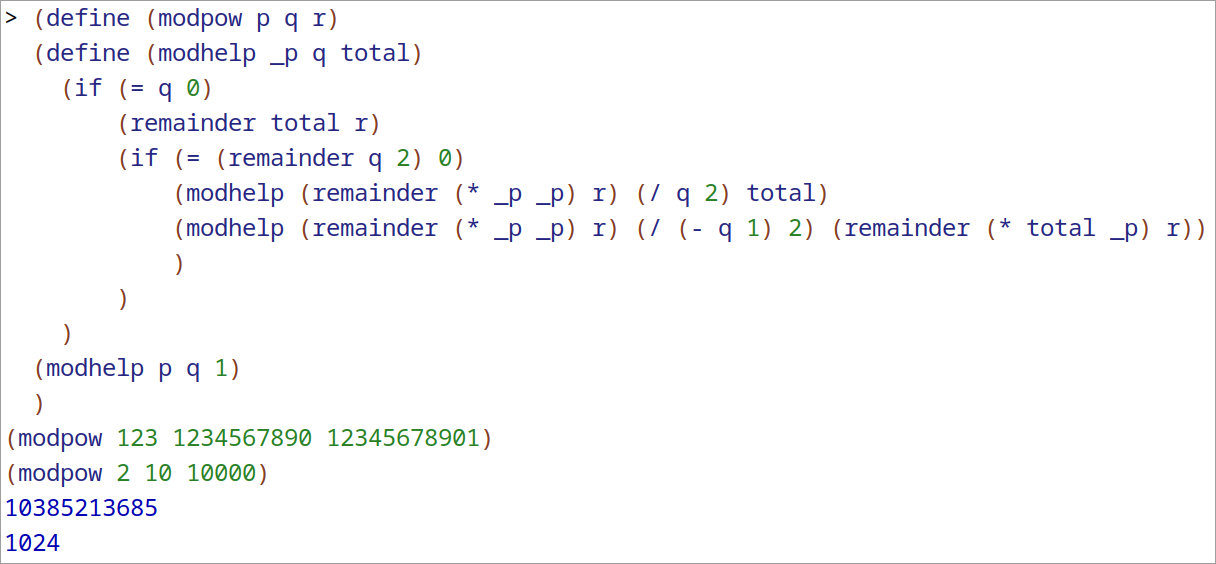
\includegraphics[scale=0.35]{modpow.png}
	\end{center}

	\newpage
	\section{}
	\begin{verbatim}
;; Notkun: (cornerstream s n)
;; Fyrir: s er óendanlegur straumur óendanlegra
;;        strauma,
;;        s=[[x11 x12 ...],[x21 x22 ...] ...].
;;        n er heiltala, n>=0.
;; Gildi: Listinn
;;        ((x11 x12 ... x1n)
;;        (x21 x22 ... x2n)
;;        ...
;;        (xn1 xn2 ... xnn)
;;        )
(define (cornerstream s n)
  ;; Notkun: (makelist substream index)
  ;; Fyrir: substream er óendanlegur straumur, [x1, x2, ...],
  ;;        index er heiltala, 0 <= index <= n
  ;; Gildi: Listinn (x1, x2, ... , x_index)
  (define (makelist substream index)
    (if (= index 0)
        '()
        (cons (stream-car substream) (makelist (stream-cdr substream) (- index 1)))
        )
    )
  ;; Notkun: (cornerhelp stream index)
  ;; Fyrir: stream er óendanlegur straumur óendanlegra
  ;;        strauma [[x11, x12, ...], [x21, x22, ...], ...],
  ;;        index er heiltala, 0 <= index <= n
  ;; Gildi: Listinn ((x11, x12, ..., x1n),
  ;;                 (x21, x22, ..., x2n),
  ;;                 ...
  ;;                 (x_index1, x_index2, ..., x_indexn))
  (define (cornerhelp stream index)
    (if (= index 0)
        '()
        (cons (makelist (stream-car stream) n) (cornerhelp (stream-cdr stream) (- index 1)))
        )
    )
  (cornerhelp s n)
  )
	\end{verbatim}
	\begin{center}
		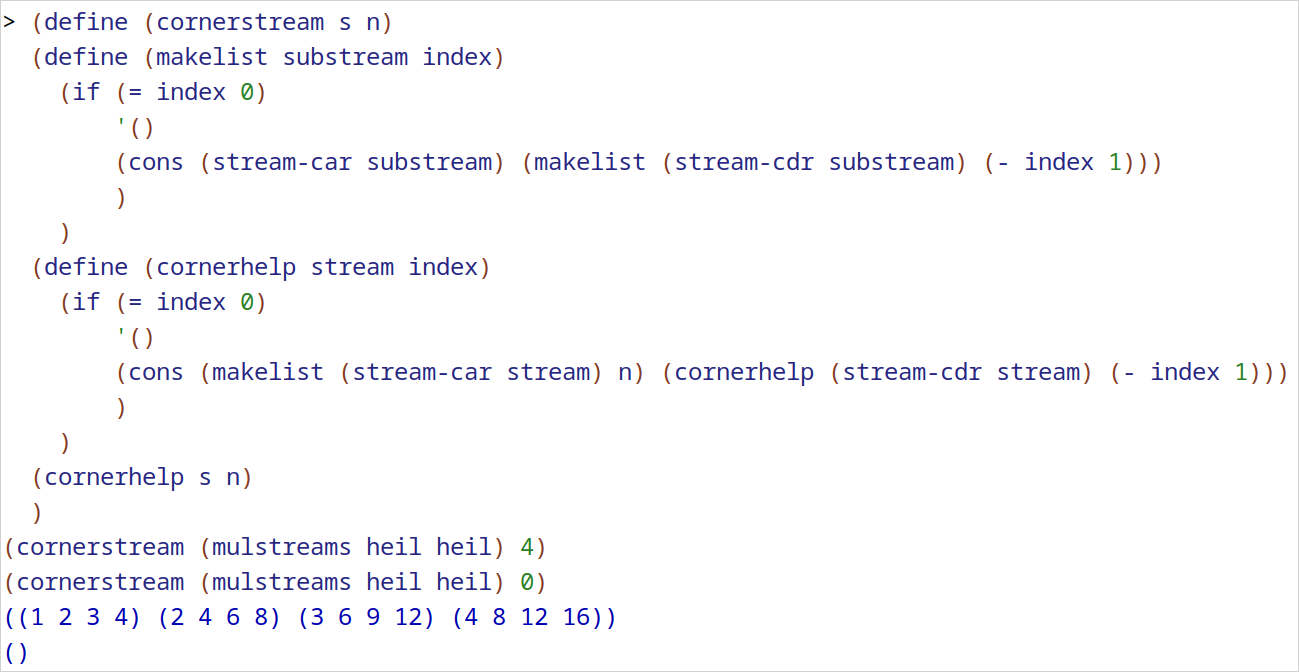
\includegraphics[scale=0.35]{cornerstream.png}
	\end{center}

	\newpage
	\section{}
	\begin{verbatim}
;; Notkun: (mulstreams x y)
;; Fyrir: x og y eru óendanlegir straumar talna,
;; x=[x1 x2 x3 ...].
;; y=[y1 y2 y3 ...].
;; Gildi: Óendanlegur straumur óendanlegra strauma
;; talna sem er
;; [[x1*y1 x2*y1 x3*y1 ...]
;; [x1*y2 x2*y2 x3*y2 ...]
;; [x1*y3 x2*y3 x3*y3 ...]
;; ...
;; ]
(define (mulstreams x y)
  ;; Notkun: (mulhelp x yval)
  ;; Fyrir: x er óendanlegur straumur talna, [x1 x2 x3 ...],
  ;;        yval er tala
  ;; Gildi: óendanlegi straumurinn [x1*yval x2*yval ...]
  (define (mulhelp x yval)
    (cons-stream (* (stream-car x) yval) (mulhelp (stream-cdr x) yval))
    )
  (cons-stream (mulhelp x (stream-car y)) (mulstreams x (stream-cdr y)))
  )
	\end{verbatim}
	\begin{center}
		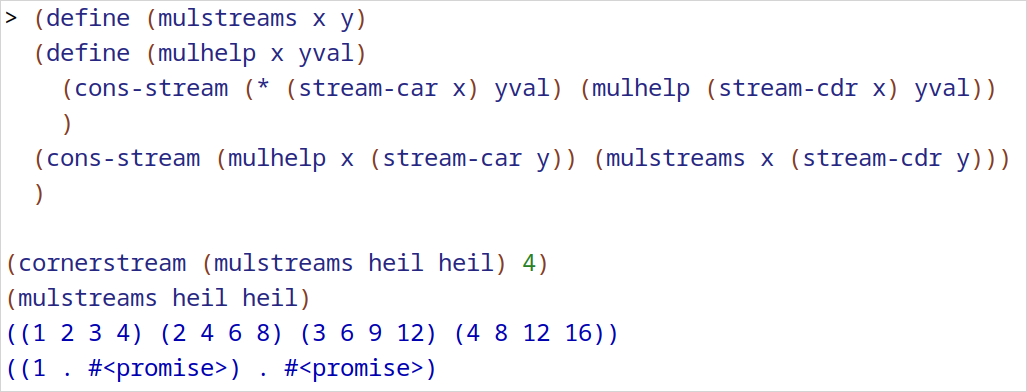
\includegraphics[scale=0.35]{mulstreams.png}
	\end{center}

	\newpage
	\section{}
	\begin{verbatim}
;; Notkun: (powerlist n)
;; Fyrir: n er heiltala, n>=0.
;; Gildi: Listinn (y1 y2 y3 ...)
;;        sem inniheldur alla lista sem
;;        hægt er að smíða með því að taka
;;        núll eða fleiri gildi úr {1,...,n}
;;        og skeyta þeim saman í lista í
;;        minnkandi röð.
(define (powerlist n)
  ;; Notkun: (addn l)
  ;; Fyrir: l er listi, l = (l1 l2 ... lm)
  ;; Gildi: Listinn (n l1 l2 ... lm)
  (define (addn l)
    (cons n l)
    )
  (if (= n 0)
      '(())
      (append (powerlist (- n 1)) (map addn (powerlist (- n 1))))
      )
  )
	\end{verbatim}
	\begin{center}
		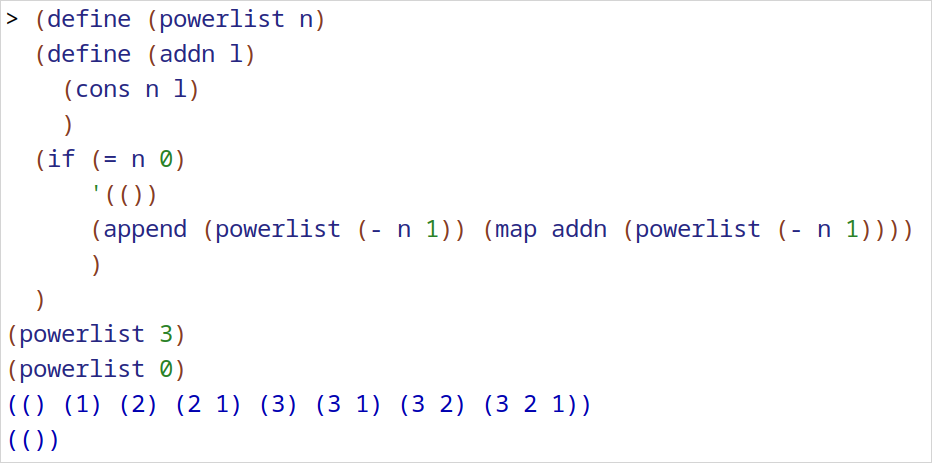
\includegraphics[scale=0.35]{powerlist.png}
	\end{center}
\end{document}
